\documentclass{article}
\usepackage[T1]{fontenc}
\usepackage{lmodern}
\usepackage{graphicx}
\usepackage{amsmath,amssymb}
\usepackage[a4paper,margin=2cm]{geometry}
\usepackage[absolute,overlay]{textpos}
\setlength{\TPHorizModule}{1mm}
\setlength{\TPVertModule}{1mm}
\usepackage[indonesian]{babel}
\usepackage{hyperref}
\setlength{\emergencystretch}{2em}
% unit: Halaman 23

\begin{document}

% === Halaman 23 (llm) ===

% (tidak ada teks dari model)

% deskripsi: Diagram hierarki klasifikasi Kriptologi yang terbagi menjadi Kriptografi dan Kriptanalisis. Kriptografi selanjutnya terbagi menjadi Cipher Simetris, Cipher Asimetris, dan Fungsi Hash. Cipher Simetris terbagi lagi menjadi Block Ciphers dan Stream Ciphers.
% bbox normalisasi: [0.1100, 0.1700, 0.7800, 0.7500]
\begin{textblock*}{140.70mm}(23.10mm,50.49mm)
\noindent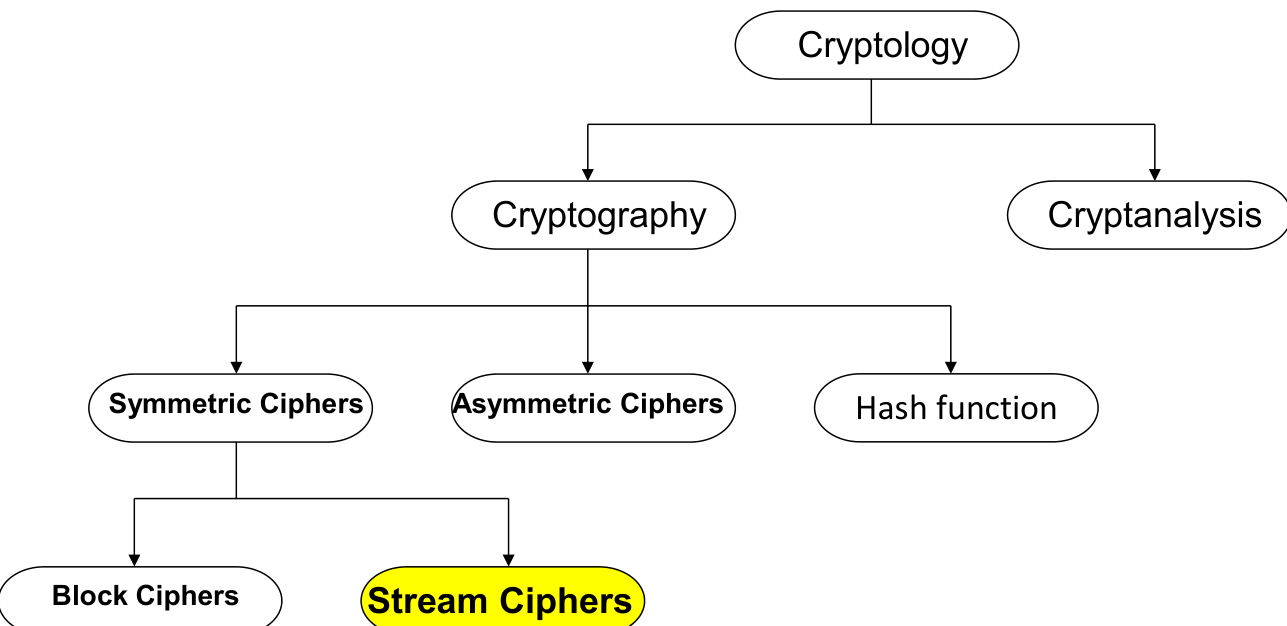
\includegraphics[width=140.70mm,height=172.26mm]{../../images/llm/page_023_img_01.png}%
\end{textblock*}

\end{document}
